% !TEX root = ../main.tex
% ============================================================================
% CAPÍTULO 5 — ANÁLISIS DE COSTOS Y PRESUPUESTO
% ============================================================================

\chapter{ANÁLISIS DE COSTOS Y PRESUPUESTO}

Este capítulo cuantifica el costo de desarrollar, fabricar y validar el sistema descrito en los Capítulos 3 y 4, y evalúa su viabilidad económica frente a alternativas comerciales existentes. El desglose sigue el mismo criterio de agrupación funcional ya establecido en la lista de materiales del Capítulo~3 (Tabla~\ref{bom}) y en la tabla de componentes del prototipo del Capítulo~4 (Tabla~\ref{tab:componentes_protoboard}). Así, cada partida de costo puede rastrearse hasta el componente físico concreto que la origina, en lugar de quedar como una cifra agregada sin respaldo.

Los montos se expresan en bolivianos (Bs), moneda de referencia ya utilizada en el resto de la tesis (por ejemplo, \texttt{FUEL\_PRICE\_BS\_PER\_L} en el firmware), con una columna equivalente en dólares (USD) para los componentes que se cotizan internacionalmente (LCSC, JLCPCB, AliExpress). Dado que el tipo de cambio BOB/USD ha tenido variaciones significativas en el mercado boliviano en los últimos años, las conversiones de este capítulo usan el tipo de cambio paralelo vigente al momento de la cotización, 11,60\,Bs/USD (agosto de 2026), y no un valor fijo asumido de antemano ni el tipo de cambio oficial, que en este periodo no refleja el costo real de acceso a dólares para la importación de componentes.

\section{Costos de componentes electrónicos}

Esta sección desglosa el costo de los componentes electrónicos en los mismos cuatro bloques funcionales de la Tabla~\ref{bom}: procesamiento, alimentación, interfaz CAN y periféricos. Las cantidades de cada fila provienen directamente de esa tabla; aquí solo se añaden el precio unitario y el subtotal por bloque.

\subsection{Costos del módulo de procesamiento (ESP32-S3)}

\begin{table}[H]
	\centering
	\captionsetup{labelformat=simple, labelsep=newline, textfont=it, labelfont=bf, justification=raggedright, singlelinecheck=false}
	\caption{Costo del módulo de procesamiento}
	\label{tab:costo_procesamiento}
	\begin{tabularx}{\textwidth}{X >{\centering\arraybackslash}p{1.6cm} >{\centering\arraybackslash}p{2.6cm} >{\centering\arraybackslash}p{2.6cm} >{\centering\arraybackslash}p{2.6cm}}
		\toprule
		\rowcolor[rgb]{0.851, 0.851, 0.851}
		Componente & Cant. & Precio unit. (USD) & Precio unit. (Bs) & Subtotal (Bs) \\
		\midrule
		Módulo ESP32-S3-WROOM-1-N16R8 (DevKitC-1, prototipo) & 1 & 9,48 & 110 & 110 \\
		\bottomrule
	\end{tabularx}
	\vspace{2mm}
	\\
	\begin{minipage}{\linewidth}
		\small
		\textit{Nota.} Precio de referencia del módulo de desarrollo completo (\textit{DevKitC-1}) usado en el prototipo sobre protoboard (Tabla~\ref{tab:componentes_protoboard}); si la versión final en PCB propia usa el módulo ESP32-S3-WROOM-1-N16R8 suelto en vez del DevKit completo, el precio unitario es menor pero requiere programador externo para el primer flasheo.
	\end{minipage}
\end{table}

\subsection{Costos de la etapa de alimentación (buck y LDOs)}

\begin{table}[H]
	\centering
	\captionsetup{labelformat=simple, labelsep=newline, textfont=it, labelfont=bf, justification=raggedright, singlelinecheck=false}
	\caption{Costo de la etapa de alimentación de dos rieles}
	\label{tab:costo_alimentacion}
	\begin{tabularx}{\textwidth}{X >{\centering\arraybackslash}p{1.6cm} >{\centering\arraybackslash}p{2.6cm} >{\centering\arraybackslash}p{2.6cm} >{\centering\arraybackslash}p{2.6cm}}
		\toprule
		\rowcolor[rgb]{0.851, 0.851, 0.851}
		Componente & Cant. & Precio unit. (USD) & Precio unit. (Bs) & Subtotal (Bs) \\
		\midrule
		Convertidor buck síncrono TPS54302DDCR & 1 & 0,2538 & 2,94 & 2,94 \\
		LDO AMS1117-3.3 (riel 1) & 1 & 0,2039 & 2,37 & 2,37 \\
		LDO AP2112K-3.3TRG1 (riel 2) & 1 & 0.2043 & 2,37 & 2,37 \\
		Diodo Schottky SS34 (protección polaridad) & 1 & 0,039 & 0,45 & 0,45 \\
		Fusible PTC reseteable 1812L150/33GR & 1 & 0,0575 & 0,67 & 0,67 \\
		Inductor de potencia 10~\textmu H & 1 & 1,3769 & 15,97 & 15,97 \\
		Condensadores y resistencias pasivas (Tabla~\ref{bom}) & 16 & 0,7323 & 8,49 & 135,91 \\
		\bottomrule
	\end{tabularx}
	\vspace{2mm}
	\\
	\begin{minipage}{\linewidth}
		\small
		\textit{Nota.} Los pasivos (condensadores, resistencias) se cotizan casi siempre por cinta/carrete completo aunque el diseño solo use unas pocas unidades; a cantidad de prototipo (1 placa), su costo unitario efectivo suele ser mayor que en producción en volumen. Es algo esperable, que debería diluirse si el proyecto escala a una serie de unidades, según se discute en la Subsección~\ref{sec:costo_beneficio}.
	\end{minipage}
\end{table}

\subsection{Costos de la interfaz CAN (transceptor y protección)}

\begin{table}[H]
	\centering
	\captionsetup{labelformat=simple, labelsep=newline, textfont=it, labelfont=bf, justification=raggedright, singlelinecheck=false}
	\caption{Costo de la interfaz de bus CAN}
	\label{tab:costo_can}
	\begin{tabularx}{\textwidth}{X >{\centering\arraybackslash}p{1.6cm} >{\centering\arraybackslash}p{2.6cm} >{\centering\arraybackslash}p{2.6cm} >{\centering\arraybackslash}p{2.6cm}}
		\toprule
		\rowcolor[rgb]{0.851, 0.851, 0.851}
		Componente & Cant. & Precio unit. (USD) & Precio unit. (Bs) & Subtotal (Bs) \\
		\midrule
		Transceptor CAN SN65HVD230 & 1 & 1,5216 & 17,65 & 17,65 \\
		Resistor control de pendiente (10~k$\Omega$) & 1 & 0,0912 & 1,06 & 1,06 \\
		Resistor de terminación 120~$\Omega$ (\textit{footprint} opcional, no poblado) & 0 & --- & --- & 0{,}00 \\
		Condensador de desacople & 1 & 0,4296 & 4,98 & 4,98 \\
		\bottomrule
	\end{tabularx}
	\vspace{2mm}
	\\
	\begin{minipage}{\linewidth}
		\small
		\textit{Nota.} El resistor de terminación no se puebla por defecto (Tabla~\ref{bom}, nota $^{a}$), ya que el dispositivo se conecta en derivación a un bus CAN que el vehículo ya termina; se incluye en la tabla únicamente para dejar registrado el criterio de costo cero de esa partida, no por omisión.
	\end{minipage}
\end{table}

\subsection{Costos de periféricos (MicroSD, OLED, conectores)}

\begin{table}[H]
	\centering
	\captionsetup{labelformat=simple, labelsep=newline, textfont=it, labelfont=bf, justification=raggedright, singlelinecheck=false}
	\caption{Costo de periféricos de almacenamiento, visualización y conexión}
	\label{tab:costo_perifericos}
	\begin{tabularx}{\textwidth}{X >{\centering\arraybackslash}p{1.6cm} >{\centering\arraybackslash}p{2.6cm} >{\centering\arraybackslash}p{2.6cm} >{\centering\arraybackslash}p{2.6cm}}
		\toprule
		\rowcolor[rgb]{0.851, 0.851, 0.851}
		Componente & Cant. & Precio unit. (USD) & Precio unit. (Bs) & Subtotal (Bs) \\
		\midrule
		Zócalo MicroSD (\textit{push-push}) & 1 & 0,1318 & 1,53 & 1,53 \\
		Tarjeta MicroSD (capacidad de referencia) & 1 & 3,2141 & 37,28 & 37,28 \\
		Pantalla OLED SSD1306 I\textsuperscript{2}C 0,96 & 1 & 2,686 & 31,16 & 31,16 \\
		Conector OBD-II tipo A con cable & 1 & 0,8 & 9,28 & 9,28 \\
		LEDs indicadores + resistencias limitadoras & 4 & 0,2120 & 2,46 & 9,84 \\
		Resistencias \textit{pull-up} SPI/I\textsuperscript{2}C (Tabla~\ref{bom}) & 6 & 0,0460 & 0,53 & 3,20 \\
		\bottomrule
	\end{tabularx}
	\vspace{2mm}
	\\
	\begin{minipage}{\linewidth}
		\small
		\textit{Nota.} La capacidad de la tarjeta MicroSD es más una decisión de autonomía de registro que de costo: dado el tamaño de fila estimado en el Capítulo~4 ($\approx$100 bytes/fila a 1 muestra/s), incluso una tarjeta de 8~GB excede ampliamente los requisitos de años de uso continuo, así que pagar por mayor capacidad no tiene sentido.
	\end{minipage}
\end{table}

\section{Costos de desarrollo y software}

El conjunto de herramientas de desarrollo empleado (Visual Studio Code, la extensión PlatformIO IDE, el \textit{framework} \texttt{arduino-esp32}, y el editor EasyEDA en su capa gratuita para el esquemático y la PCB) es de uso libre y sin costo de licenciamiento, criterio de selección ya justificado en la Sección de herramientas del Capítulo~3. El costo real de esta partida no está en licencias, entonces, sino en el tiempo de ingeniería invertido en el diseño de hardware, el firmware y la interfaz web.

\begin{table}[H]
	\centering
	\captionsetup{labelformat=simple, labelsep=newline, textfont=it, labelfont=bf, justification=raggedright, singlelinecheck=false}
	\caption{Costo estimado de horas de ingeniería por etapa de desarrollo}
	\label{tab:costo_horas}
	\begin{tabularx}{\textwidth}{X >{\centering\arraybackslash}p{2.6cm} >{\centering\arraybackslash}p{2.6cm} >{\centering\arraybackslash}p{2.6cm}}
		\toprule
		\rowcolor[rgb]{0.851, 0.851, 0.851}
		Etapa & Horas estimadas & Tarifa (Bs/h) & Subtotal (Bs) \\
		\midrule
		Diseño de esquemático y PCB & 8 & 0 & 0 \\
		Desarrollo de firmware (adquisición, cálculo, almacenamiento) & 28 & 0 & 0 \\
		Desarrollo del panel web (HMI) & 28 & 0 & 0 \\
		Pruebas, calibración y depuración & 120 & 0 & 0 \\
		\midrule
		\textbf{Total} & \textbf{184} & --- & \textbf{0} \\
		\bottomrule
	\end{tabularx}
	\vspace{2mm}
	\\
	\begin{minipage}{\linewidth}
		\small
		\textit{Nota.} Horas estimadas a partir de la dedicación real registrada por el autor ($\approx$4\,h/día): 2 días (PCB), 1 semana (firmware y panel web, 7 días cada uno) y 1 mes (calibración, 30 días). La tarifa se deja en 0\,Bs/h a propósito. Este capítulo lo permite porque el objetivo es el costo de materiales y fabricación, no el valor de mercado de las horas de un proyecto de grado; el total de 184\,h queda documentado como referencia de esfuerzo, no como partida monetaria del presupuesto.
	\end{minipage}
\end{table}

\section{Costos de fabricación y ensamblaje}

\subsection{Costos de la placa preliminar (Robokit)}
\label{sec:costo_pcb_preliminar}

La placa preliminar en EasyEDA descrita en la Sección~\ref{sec:placa_preliminar} (Capítulo~4) es, hasta el momento, la única placa de este proyecto efectivamente fabricada y ensamblada; por eso es la que se usa como \textbf{costo real del prototipo} en el presupuesto consolidado de este capítulo (Tabla~\ref{tab:presupuesto_total}). Se encargó localmente a Robokit (La Paz), lo que evita el envío internacional y la aduana que sí aplican a una fabricación en JLCPCB (Subsección~\ref{sec:costo_pcb_final}).

\begin{table}[H]
	\centering
	\captionsetup{labelformat=simple, labelsep=newline, textfont=it, labelfont=bf, justification=raggedright, singlelinecheck=false}
	\caption{Costo de fabricación de la placa preliminar en Robokit}
	\label{tab:costo_pcb_preliminar}
	\begin{tabularx}{\textwidth}{X >{\centering\arraybackslash}p{2cm} >{\centering\arraybackslash}p{2.6cm}}
		\toprule
		\rowcolor[rgb]{0.851, 0.851, 0.851}
		Concepto & Cantidad & Subtotal (Bs) \\
		\midrule
		Fabricación de PCB (Robokit, La Paz) & 1 & 150,00 \\
		Ensamblaje (soldadura manual, propia) & --- & 0,00 \\
		\midrule
		\textbf{Total} & --- & \textbf{150,00} \\
		\bottomrule
	\end{tabularx}
	\vspace{2mm}
	\\
	\begin{minipage}{\linewidth}
		\small
		\textit{Nota.} Cotización y fabricación locales (La Paz), sin envío internacional ni aduana. El ensamblaje fue realizado por el propio autor, por lo que no tiene costo monetario adicional, consistente con el criterio ya aplicado en la Tabla~\ref{tab:costo_horas} (tarifa de horas propias en 0\,Bs/h).
	\end{minipage}
\end{table}

La lista de materiales real de esta placa (16 referencias, exportada desde EasyEDA) muestra que su etapa de alimentación es una regulación lineal simple (7805 + transistor de paso TIP42C) y no la conversión conmutada de dos rieles de la Tabla~\ref{tab:costo_alimentacion} —esa etapa es específica de la placa final—; el módulo ESP32-S3, el transceptor CAN, la pantalla OLED y la tarjeta microSD son los mismos ya presupuestados en las Tablas~\ref{tab:costo_procesamiento}, \ref{tab:costo_can} y~\ref{tab:costo_perifericos}, reutilizados desde la etapa de protoboard y conectados a esta placa mediante los conectores de la Tabla~\ref{tab:costo_placa_preliminar_bom} en vez de cableado suelto. Los indicadores LED y sus resistencias limitadoras también coinciden con los ya contabilizados en la Tabla~\ref{tab:costo_perifericos}, por lo que no se repiten aquí.

\begin{table}[H]
	\centering
	\captionsetup{labelformat=simple, labelsep=newline, textfont=it, labelfont=bf, justification=raggedright, singlelinecheck=false}
	\caption{Componentes adicionales de la placa preliminar (etapa de alimentación y conectores)}
	\label{tab:costo_placa_preliminar_bom}
	\begin{tabularx}{\textwidth}{X >{\centering\arraybackslash}p{1.6cm} >{\centering\arraybackslash}p{2.2cm} >{\centering\arraybackslash}p{2.2cm} >{\centering\arraybackslash}p{2.2cm}}
		\toprule
		\rowcolor[rgb]{0.851, 0.851, 0.851}
		Componente & Cant. & Precio unit. (USD) & Precio unit. (Bs) & Subtotal (Bs) \\
		\midrule
		Regulador lineal 7805 (TO-252) & 1 & 0,0979 & 1,14 & 1,14 \\
		Transistor de paso TIP42C (TO-220) & 1 & 0,1777 & 2,06 & 2,06 \\
		Capacitor electrolítico 220\,\textmu F & 1 & 0,1400 & 1,62 & 1,62 \\
		Capacitor electrolítico 22\,\textmu F & 1 & 0,1200 & 1,39 & 1,39 \\
		Capacitor cerámico 100\,nF & 2 & 0,0200 & 0,23 & 0,46 \\
		Resistor THT 47\,$\Omega$ 1\,W & 1 & 0,0112 & 0,13 & 0,13 \\
		Conector de entrada de alimentación, 4~pines (WJ301V-5.0) & 1 & 0,1700 & 1,97 & 1,97 \\
		Header 4~pines (pantalla OLED) & 1 & 0,0198 & 0,23 & 0,23 \\
		Header 6~pines (transceptor SN65HVD230) & 1 & 0,0298 & 0,35 & 0,35 \\
		Header 8~pines (módulo microSD) & 1 & 0,0400 & 0,46 & 0,46 \\
		\midrule
		\textbf{Total} & --- & --- & --- & \textbf{9,81} \\
		\bottomrule
	\end{tabularx}
	\vspace{2mm}
	\\
	\begin{minipage}{\linewidth}
		\small
		\textit{Nota.} Precios de referencia LCSC para las referencias de fabricante exportadas desde EasyEDA (por ejemplo, \texttt{KS104M050C07RR0VH2FP0} para el capacitor de 100\,nF), convertidos a bolivianos al tipo de cambio de este capítulo (11,60\,Bs/USD); las referencias sin coincidencia exacta en el catálogo (capacitor de 22\,\textmu F, header de 8 pines y conector de 4 pines) se estiman por interpolación directa a partir de variantes de la misma familia con precio confirmado (por ejemplo, el conector WJ301V-5.0 sí tiene precio publicado en sus variantes de 2 y 3 pines), no por un valor arbitrario.
	\end{minipage}
\end{table}

\subsection{Costos de manufactura de la placa final (JLCPCB)}
\label{sec:costo_pcb_final}

A diferencia de la placa preliminar, la placa final documentada en el Capítulo~3 (diseñada en Altium Designer) todavía no se ha mandado a fabricar; esta subsección presenta su cotización de referencia, relevante si el proyecto avanza hacia esa versión más profesional o hacia una serie piloto para varios vehículos de transporte público. Se cotiza sobre el lote mínimo estándar de JLCPCB para placas de dos capas (Tabla~\ref{jlcpcb}, Capítulo~3), habitualmente de 5 unidades, que es también el tamaño de lote recomendado para tener margen ante fallas de soldadura o defectos de una unidad individual durante las pruebas iniciales.

\begin{table}[H]
	\centering
	\captionsetup{labelformat=simple, labelsep=newline, textfont=it, labelfont=bf, justification=raggedright, singlelinecheck=false}
	\caption{Costo de fabricación de PCB en JLCPCB}
	\label{tab:costo_pcb}
	\begin{tabularx}{\textwidth}{X >{\centering\arraybackslash}p{1.6cm} >{\centering\arraybackslash}p{2.2cm} >{\centering\arraybackslash}p{2.2cm} >{\centering\arraybackslash}p{2.2cm}}
		\toprule
		\rowcolor[rgb]{0.851, 0.851, 0.851}
		Concepto & Cantidad & Precio unit. (USD) & Precio unit. (Bs) & Subtotal (Bs) \\
		\midrule
		Fabricación de PCB (lote mínimo, 2 capas, 1~oz) & 1 & 4,00 & 46,40 & 46,40 \\
		Envío internacional (DHL/courier) & 1 & 38,00 & 440,80 & 440,80 \\
		Impuestos/aduana de importación (si aplica) & 1 & - & - & - \\
		\bottomrule
	\end{tabularx}
	\vspace{2mm}
	\\
	\begin{minipage}{\linewidth}
		\small
		\textit{Nota.} El envío y la aduana suelen pesar más en el costo total que la fabricación misma para lotes de prototipo pequeños importados a Bolivia; conviene cotizar ambos conceptos por separado y no asumir que están incluidos en el precio de fabricación publicado por JLCPCB.
	\end{minipage}
\end{table}

\subsection{Costos de ensamblaje SMD de la placa final}

Para la placa final, el ensamblaje de los componentes de montaje superficial puede resolverse por dos vías con una disyuntiva clara de costo contra riesgo: el servicio de ensamblaje (PCBA) del propio fabricante, o el soldado manual con estación de aire caliente/soldadora de precisión. La placa preliminar (Sección~\ref{sec:costo_pcb_preliminar}), en cambio, ya se ensambló manualmente por el propio autor, sin necesidad de esta disyuntiva.

\begin{table}[H]
	\centering
	\captionsetup{labelformat=simple, labelsep=newline, textfont=it, labelfont=bf, justification=raggedright, singlelinecheck=false}
	\caption{Comparación de estrategias de ensamblaje SMD}
	\label{tab:costo_ensamblaje}
	\begin{tabularx}{\textwidth}{>{\raggedright\arraybackslash}p{3.2cm} X X}
		\toprule
		\rowcolor[rgb]{0.851, 0.851, 0.851}
		Criterio & Ensamblaje PCBA (JLCPCB) & Soldadura manual \\
		\midrule
		Costo & 1\,440,60 Bs (124,19 USD; incluye \textit{setup} + componentes + mano de obra) & Solo costo de componentes; tiempo propio no facturado \\
		Riesgo técnico & Bajo: máquina \textit{pick-and-place} coloca el TPS54302DDCR (SOT-23-6) sin riesgo de puente de soldadura & Medio-alto en los pasivos 0603 y el regulador \textit{buck}, componentes de paso fino \\
		Tiempo de entrega & Sujeto al lote de fabricación + envío & Inmediato una vez recibida la PCB desnuda \\
		Recomendado cuando & Se fabrica más de una unidad, o no se dispone de estación de retrabajo SMD & Se ensambla una sola unidad de prototipo y ya se cuenta con el equipo de soldadura \\
		\bottomrule
	\end{tabularx}
	\vspace{2mm}
	\\
	\begin{minipage}{\linewidth}
		\small
		\textit{Nota.} Elaboración propia. Comparación de referencia para cuando se mande a fabricar la placa final; la vía efectivamente utilizada para la placa preliminar ya construida (Tabla~\ref{tab:costo_pcb_preliminar}) fue la soldadura manual (columna derecha), con el mismo criterio de costo cero de mano de obra propia que el resto del capítulo.
	\end{minipage}
\end{table}

\section{Costos de pruebas y validación}

\begin{table}[H]
	\centering
	\captionsetup{labelformat=simple, labelsep=newline, textfont=it, labelfont=bf, justification=raggedright, singlelinecheck=false}
	\caption{Costos asociados a la fase de pruebas y validación (Capítulo 4)}
	\label{tab:costo_pruebas}
	\begin{tabularx}{\textwidth}{X >{\centering\arraybackslash}p{2.6cm} >{\centering\arraybackslash}p{2.6cm} >{\centering\arraybackslash}p{2.6cm}}
		\toprule
		\rowcolor[rgb]{0.851, 0.851, 0.851}
		Concepto & Cantidad & Precio unit. (Bs) & Subtotal (Bs) \\
		\midrule
		Adaptador ELM327 Bluetooth (referencia de validación) & 1 & 85,00 & 85,00 \\
		Suscripción \textit{Car Scanner} Premium (3 meses) & 1 & 22,99 & 22,99 \\
		Combustible para trayectos de prueba tanque a tanque (Sección~\ref{sec:protocolo_tanque}, Cap.~4) & 22,03~L & 6,96 & 153,33 \\
		Instrumento de medición de corriente (tester) & 1 & 55,00 & 55,00 \\
		\midrule
		\textbf{Total} & --- & --- & \textbf{316,32} \\
		\bottomrule
	\end{tabularx}
	\vspace{2mm}
	\\
	\begin{minipage}{\linewidth}
		\small
		\textit{Nota.} El precio del litro de gasolina (6,96~Bs) es el mismo valor de referencia (\texttt{FUEL\_PRICE\_BS\_PER\_L}) que usa el propio firmware para calcular el costo acumulado del viaje (Capítulo~3), de modo que lo que reporta el dispositivo en campo y lo que presupuesta este capítulo quedan alineados. Los 22,03~L de combustible son la suma de los dos totales reales de aforo tanque lleno del Capítulo~4 (Nissan Vanette 12,96~L + Changan Honor 9,07~L, Tablas~\ref{tab:comparacion_consumo_vanette}/\ref{tab:comparacion_consumo_changan}): el consumo efectivamente gastado en los nueve tramos de prueba de ambos vehículos, no la capacidad de los tanques.
	\end{minipage}
\end{table}

\section{Presupuesto total del proyecto}

La Tabla~\ref{tab:presupuesto_total} consolida los subtotales de las secciones anteriores, usando la placa preliminar de Robokit (Sección~\ref{sec:costo_pcb_preliminar}) como fabricación real del prototipo. El presupuesto se presenta también en su forma de \textit{costo marginal por unidad adicional} (Tabla~\ref{tab:presupuesto_total}, última fila), escalando esta vez hacia la placa final en Altium Designer y su fabricación en JLCPCB (Sección~\ref{sec:costo_pcb_final}), relevante si el proyecto avanza hacia esa versión más profesional o hacia una pequeña serie de dispositivos para varios vehículos de transporte público, escenario directamente ligado a la motivación planteada en el Capítulo~1.

\begin{table}[H]
	\centering
	\captionsetup{labelformat=simple, labelsep=newline, textfont=it, labelfont=bf, justification=raggedright, singlelinecheck=false}
	\caption{Presupuesto total del proyecto, por categoría}
	\label{tab:presupuesto_total}
	\begin{tabularx}{\textwidth}{X >{\centering\arraybackslash}p{3.5cm} >{\centering\arraybackslash}p{3cm}}
		\toprule
		\rowcolor[rgb]{0.851, 0.851, 0.851}
		Categoría & Subtotal (Bs) & \%~del total \\
		\midrule
		Componentes electrónicos (Tablas~\ref{tab:costo_procesamiento}, \ref{tab:costo_can}, \ref{tab:costo_perifericos} y~\ref{tab:costo_placa_preliminar_bom}) & 235,79 & 33,58\,\% \\
		Desarrollo y software (Tabla~\ref{tab:costo_horas}) & 0,00 & 0,00\,\% \\
		Fabricación y ensamblaje, placa preliminar (Tabla~\ref{tab:costo_pcb_preliminar}) & 150,00 & 21,36\,\% \\
		Pruebas y validación (Tabla~\ref{tab:costo_pruebas}) & 316,32 & 45,05\,\% \\
		\midrule
		\textbf{Total del prototipo} & \textbf{702,11} & \textbf{100\,\%} \\
		\midrule
		Costo marginal estimado por unidad adicional, placa final$^{a}$ & 772,22 & --- \\
		\bottomrule
	\end{tabularx}
	\vspace{2mm}
	\\
	\begin{minipage}{\linewidth}
		\small
		\textit{Nota.} $^{a}$A diferencia del total del prototipo (que usa la placa preliminar de Robokit, ya fabricada), esta fila estima el costo de una unidad adicional producida por la vía de la placa final: excluye las horas de diseño de hardware/firmware (Tabla~\ref{tab:costo_horas}), que son un costo de desarrollo único (\textit{non-recurring engineering}) y no se repiten por unidad adicional fabricada. Incluye componentes (386,66\,Bs) más la fabricación de PCB y el ensamblaje PCBA a prorrata del lote mínimo de 5 unidades de JLCPCB (Tablas~\ref{tab:costo_pcb}/\ref{tab:costo_ensamblaje}: $(487{,}20+1\,440{,}60)/5 = 385{,}56$\,Bs), es decir $386{,}66+385{,}56=772{,}22$\,Bs por unidad adicional dentro del mismo lote.
	\end{minipage}
\end{table}

\begin{figure}[H]
	\centering
	\caption{Distribución porcentual del presupuesto total del proyecto por categoría}
	\label{fig:pastel_presupuesto}
	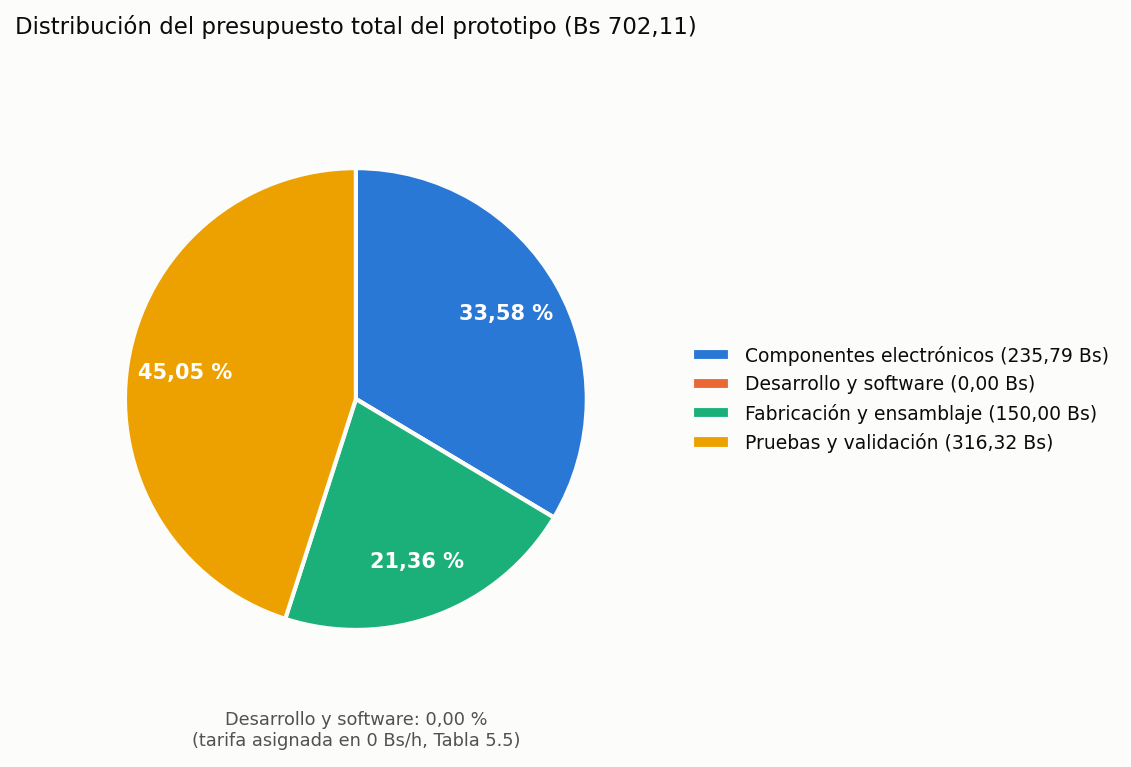
\includegraphics[width=0.85\textwidth]{Images/figura_presupuesto_pastel.png}

	\vspace{2pt}
	{\footnotesize\textit{Nota.} Se elige un gráfico de pastel porque las cuatro categorías son mutuamente excluyentes y suman el 100\,\% de un mismo presupuesto total; este tipo de gráfico comunica de forma directa qué proporción del gasto corresponde a componentes frente a mano de obra de desarrollo; una tabla de números no se lee con la misma claridad de un vistazo. Elaboración propia a partir de \texttt{CODIGOS/presupuesto\_pie.py} \citep{CalleGitHub2026}.}
\end{figure}

\section{Análisis de viabilidad económica}

\subsection{Comparación con soluciones comerciales existentes}

El sistema propuesto se contrasta contra dos categorías de alternativas ya mencionadas en los Antecedentes del Capítulo~1: los adaptadores OBD-II genéricos de bajo costo combinados con una aplicación móvil (por ejemplo, ELM327 + \textit{Car Scanner}, ya usado como referencia de validación en el Capítulo~4), y las plataformas de telemetría de flota comerciales orientadas a empresas de transporte.

\begin{table}[H]
	\centering
	\captionsetup{labelformat=simple, labelsep=newline, textfont=it, labelfont=bf, justification=raggedright, singlelinecheck=false}
	\caption{Comparación funcional y de costo frente a alternativas comerciales}
	\label{tab:comparacion_comercial}
	\begin{tabularx}{\textwidth}{>{\raggedright\arraybackslash}p{3.4cm} X X X}
		\toprule
		\rowcolor[rgb]{0.851, 0.851, 0.851}
		Criterio & Sistema propuesto & ELM327 + app comercial & Telemetría de flota comercial \\
		\midrule
		Costo inicial & 772,22 Bs$^{a}$ (Tabla~\ref{tab:presupuesto_total}) & 85,00 Bs (Tabla~\ref{tab:costo_pruebas}) & Desde 58\,000 Bs$^{b}$ (USD 5\,000, \textit{FuelForce}, pago único); el resto de proveedores cobra el hardware por separado, sin monto público \\
		Costo recurrente & Ninguno (sin suscripción) & Suscripción \textit{Car Scanner} Premium: 22,99\,Bs cada 3 meses & USD 4 a 100 por vehículo/mes según proveedor$^{b}$ ($\approx$46 a 1\,160\,Bs/mes) \\
		Registro local sin conexión a internet & Sí (microSD) & Depende de la app & Generalmente requiere conectividad \\
		Panel propio, sin dependencia de un tercero & Sí (SoftAP local) & No (depende del proveedor de la app) & No (plataforma del proveedor) \\
		Código y diseño abiertos, personalizables & Sí & No & No \\
		Corrección/\allowbreak calibración específica del vehículo & Sí (\texttt{FUEL\_\allowbreak CALIBRATION\_\allowbreak FACTOR}, tabla VE) & Limitada o inexistente & Variable según proveedor \\
		\bottomrule
	\end{tabularx}
	\vspace{2mm}
	\\
	\begin{minipage}{\linewidth}
		\small
		\textit{Nota.} Elaboración propia. $^{a}$Se usa el costo marginal por unidad adicional escalando a la placa final (Tabla~\ref{tab:presupuesto_total}) y no el presupuesto total del prototipo (702,11\,Bs, fabricado con la placa preliminar de Robokit), porque este segundo aún incluye los instrumentos de prueba del Capítulo~4 (ELM327, tester, combustible de validación) —costos de validación, no de una unidad desplegable—, mientras que la cifra de la placa final sí representa lo que costaría producir una unidad adicional a mayor escala, con un acabado más cercano al de un producto terminado y comparable con las alternativas comerciales de esta tabla. $^{b}$Precios de mercado internacional (no existe cotización pública para el mercado boliviano), tomados de \textit{Fleetio}, ``6 Best Fuel Monitoring Systems: 2025 Comparison Guide'' (\texttt{fleetio.com/blog/fuel-monitoring-systems}, consultado en agosto de 2026): Fleetio USD 4--10/vehículo/mes; Motive desde USD~25/vehículo/mes más costo de dispositivos ELD; Samsara USD 27--33/vehículo/mes (software; hardware facturado aparte); Geotab USD 35--100/vehículo/mes (software; hardware facturado aparte); FuelForce desde USD~5\,000 en modalidad de pago único por funcionalidad, en vez de suscripción. La conversión a bolivianos usa el mismo tipo de cambio de este capítulo (11,60\,Bs/USD).
	\end{minipage}
\end{table}

\begin{figure}[H]
	\centering
	\caption{Comparación de costo inicial entre el sistema propuesto y alternativas comerciales}
	\label{fig:barras_comparacion_comercial}
	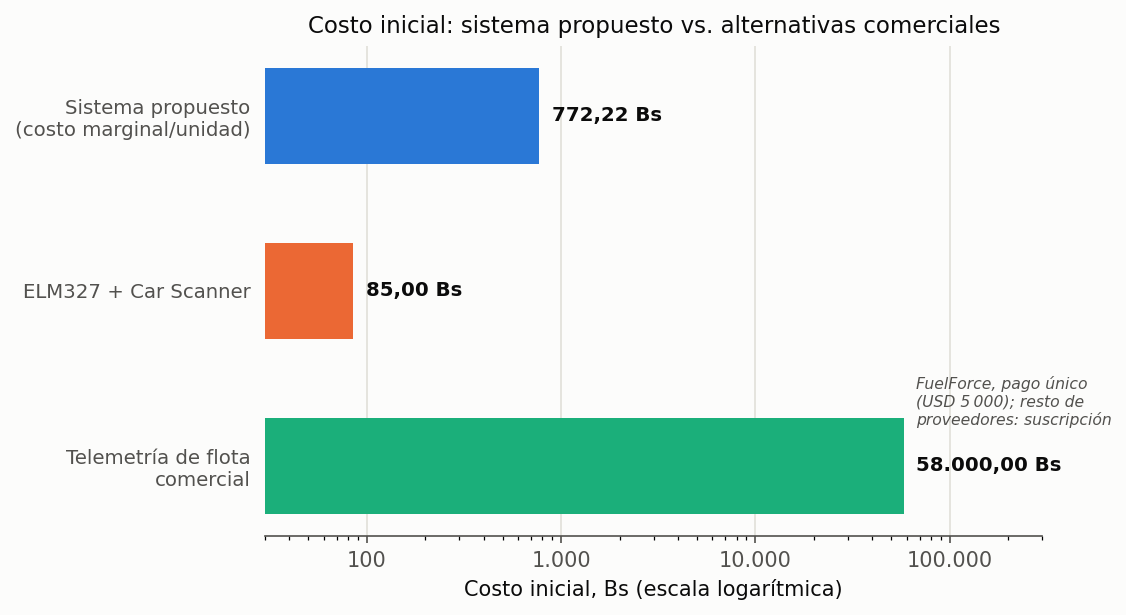
\includegraphics[width=0.85\textwidth]{Images/figura_comparacion_comercial.png}

	\vspace{2pt}
	{\footnotesize\textit{Nota.} Se elige un gráfico de barras horizontales, en vez de uno vertical, porque los nombres de las tres alternativas comparadas son largos y se leen mejor como etiquetas de eje horizontal; al ser solo tres categorías discretas comparadas por una única magnitud (costo), la barra es más directa de leer que un gráfico de líneas o de dispersión. El eje de costo usa escala logarítmica porque los tres valores abarcan casi tres órdenes de magnitud (85 a 58\,000\,Bs); cada barra conserva su valor exacto como etiqueta directa para que la escala no distorsione la lectura del monto real. El valor de telemetría de flota corresponde a un único proveedor (\textit{FuelForce}, pago único; Tabla~\ref{tab:comparacion_comercial}) y no a un promedio del rubro, ya que el resto de proveedores citados cobra por suscripción con hardware facturado aparte. Elaboración propia.}
\end{figure}

\subsection{Análisis costo-beneficio}
\label{sec:costo_beneficio}

El beneficio económico del sistema no proviene de evitar un gasto de compra (como en la comparación anterior), sino de la reducción de consumo de combustible que su uso puede inducir en el conductor al hacer visible, en tiempo real, un comportamiento de manejo ineficiente. El mecanismo exacto por el que un sistema de monitoreo reduce el consumo es de naturaleza conductual (retroalimentación al conductor) y no una modificación mecánica del vehículo, así que su magnitud solo puede estimarse una vez completada la comparación de consumo del Capítulo~4 (Tablas~\ref{tab:comparacion_consumo_vanette} y~\ref{tab:comparacion_consumo_changan}) entre trayectos con y sin atención activa al panel del dispositivo.

El periodo de recuperación de la inversión (\textit{payback period}) se estima como:

\begin{equation}
	T_{recuperación}\,[\text{meses}] = \frac{\text{Costo total del prototipo (Tabla~\ref{tab:presupuesto_total})}}{\text{Ahorro mensual estimado}\,[\text{Bs/mes}]}
	\label{eq:payback}
\end{equation}

donde el ahorro mensual se obtiene de multiplicar la reducción porcentual de consumo por retroalimentación al conductor (valor de literatura, ya que no se midió en este proyecto) por el gasto mensual de combustible típico del vehículo evaluado, a su vez estimado a partir del kilometraje mensual habitual (también de literatura) y el consumo promedio real observado en el Capítulo~4 (totales de aforo de las Tablas~\ref{tab:comparacion_consumo_vanette}/\ref{tab:comparacion_consumo_changan}).

\begin{table}[H]
	\centering
	\captionsetup{labelformat=simple, labelsep=newline, textfont=it, labelfont=bf, justification=raggedright, singlelinecheck=false}
	\caption{Estimación del periodo de recuperación de la inversión}
	\label{tab:payback}
	\begin{tabularx}{\textwidth}{X >{\centering\arraybackslash}p{3.5cm} >{\centering\arraybackslash}p{3.5cm}}
		\toprule
		\rowcolor[rgb]{0.851, 0.851, 0.851}
		Variable & Changan Honor & Nissan Vanette \\
		\midrule
		Kilometraje mensual estimado (km)$^{a}$ & 6\,000 & 6\,000 \\
		Consumo promedio (L/100\,km, Cap.~4)$^{b}$ & 7,94 & 10,43 \\
		Gasto mensual de combustible (Bs) & 3\,315,74 & 4\,355,57 \\
		Reducción de consumo atribuible al monitoreo (\%)$^{c}$ & 6,6 & 6,6 \\
		Ahorro mensual estimado (Bs/mes) & 218,84 & 287,47 \\
		Periodo de recuperación (meses) & 3,21 & 2,44 \\
		\bottomrule
	\end{tabularx}
	\vspace{2mm}
	\\
	\begin{minipage}{\linewidth}
		\small
		\textit{Nota.} $^{a}$No se midió el kilometraje real de estos vehículos: se usa un valor representativo (200\,km/día $\times$ 30 días) dentro del rango de 150 a 300\,km/día que reporta la literatura de operación de buses urbanos en servicio de todo el día \citep{PPIAF_UrbanBusToolkit_kpvpd}, igual para ambos vehículos al no existir un dato diferenciado por unidad. $^{b}$Consumo real de referencia (tanque lleno, no la estimación del sistema propio): total de aforo entre distancia total recorrida en los nueve tramos de prueba (Tablas~\ref{tab:comparacion_consumo_vanette}/\ref{tab:comparacion_consumo_changan}, Capítulo~4): Nissan Vanette $12{,}96/124{,}26\times100$; Changan Honor $9{,}07/114{,}25\times100$. $^{c}$La fila de reducción de consumo es la variable crítica de esta tabla y no se midió en este proyecto (requeriría un diseño experimental adicional al del Capítulo~4, por ejemplo contrastar el mismo trayecto con el panel visible frente al panel oculto para el conductor); se usa en su lugar el efecto promedio reportado por un metaanálisis de 17 estudios sobre sistemas de retroalimentación \textit{eco-driving} a bordo, $6{,}6\,\%$ de mejora en economía de combustible \citep{Sanguinetti2020EcoDriving}, dejando explícito que es un valor de literatura y no una medición propia.
	\end{minipage}
\end{table}

\begin{figure}[H]
	\centering
	\caption{Punto de equilibrio (\textit{breakeven}) entre el costo del dispositivo y el ahorro acumulado de combustible}
	\label{fig:breakeven}
	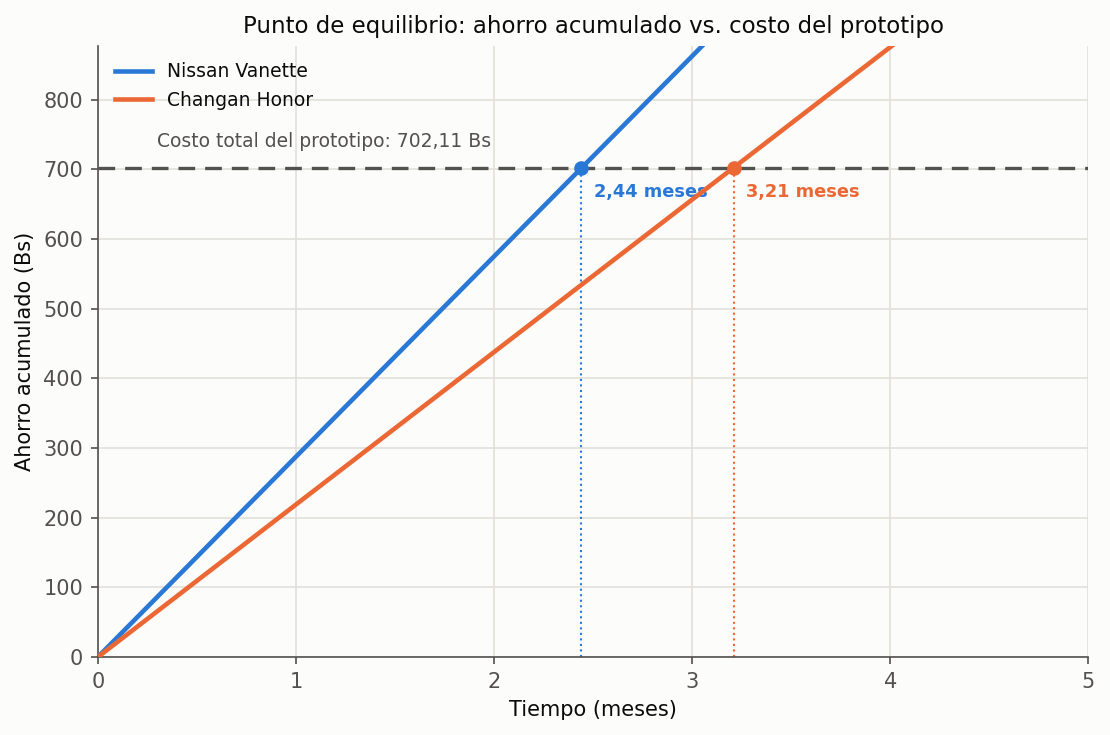
\includegraphics[width=0.85\textwidth]{Images/figura_breakeven.png}

	\vspace{2pt}
	{\footnotesize\textit{Nota.} Se elige un gráfico de líneas porque ambas magnitudes (costo fijo y ahorro acumulado) son funciones continuas del tiempo, y lo relevante para el lector es identificar visualmente el punto de cruce entre ambas curvas, algo que una tabla de valores puntuales no comunica con la misma inmediatez. Las rectas de ahorro acumulado y los periodos de recuperación (2,44 y 3,21 meses) se derivan del costo real del prototipo con la placa preliminar (Tabla~\ref{tab:presupuesto_total}) y de los valores de literatura de la Tabla~\ref{tab:payback} (kilometraje mensual y reducción de consumo atribuible al monitoreo); estos últimos no son una medición directa y el resultado debe leerse como una estimación, no como una garantía de recuperación en ese plazo exacto. Elaboración propia.}
\end{figure}

La viabilidad económica de este proyecto, para cerrar el capítulo, no depende únicamente de recuperar el costo de un prototipo individual: depende de su potencial de escalar a una pequeña serie de unidades para el transporte público de La Paz. En ese escenario, el costo marginal por unidad (Tabla~\ref{tab:presupuesto_total}), ya sin las horas de diseño amortizadas por este primer desarrollo, es la cifra económicamente relevante, y no el presupuesto total del prototipo aquí calculado.
